\section{}
Consider the simplified closed-loop diagram
\begin{figure}[h]
    \centering
    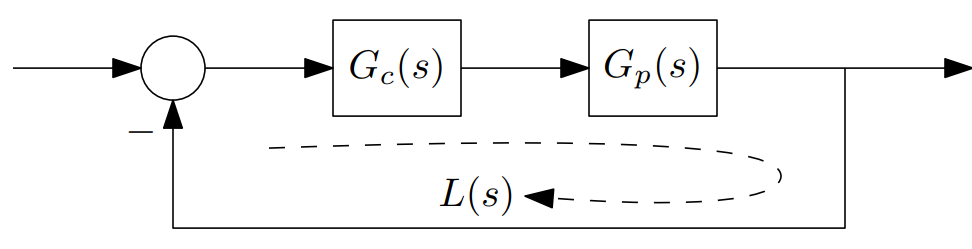
\includegraphics[width=0.5\textwidth]{Questions/Figures/Q1ProblemDiagram.png}
\end{figure}
where
\begin{equation*}
    G_c(s) = 1, \quad G_p(s) = \frac{1}{s+1}
\end{equation*}
\begin{enumerate}[label=(\alph*)]
    \item By hand, sketch the Nyquist plot of $L(s) = G_p(s)G_c(s)$. Provide both the Nyquist contour $\mathcal{D}$ and the Nyquist plot $\mathcal{G}$, 
    and label the segment endpoints $A$, $B$ and $C$.
    \item Use MATLAB's \texttt{nyquist} command to check your answer in (a). Provide the MATLAB commands you used to obtain this (you do not need to include the plot)
    \item Apply Theorem 5.3.1 (Nyquist Stability Criterion) to the above to check the stability of the closed-loop system.
    \item Now form the characteristic polynomial of the above system, and use Theorem 4.4.1 to check closed-loop stability. Does your answer match with (c)?
\end{enumerate}

\subsection{}
The loop transfer function $L(s)$ is given by
\begin{equation*}
    L(s) = G_p(s)G_c(s) = \frac{1}{s+1}
\end{equation*}
Desmos will be used to "sketch" the Nyquist plot since I'm bad at drawing with a mouse. Since $L(s)$ has real 
constant coefficients, the curve will be symmetric about the real axis. 

From $a$ to $b$, $s = j \omega$, $\omega \in [0, \infty)$, 
\begin{align*}
    L(j \omega) &= \frac{1}{j \omega + 1} \\
    &= \frac{1 - j \omega}{1 + \omega^2} 
\end{align*}
which results in 
\begin{equation*}
    \text{Re} \left\{ L(j \omega) \right\} = \frac{1}{1 + \omega^2}, \quad \text{Im} \left\{ L(j \omega) \right\} = -\frac{\omega}{1 + \omega^2}
\end{equation*}
Observe that at $\omega = 0$, $L(0) = 1$, and as $\omega \to \infty$, $L(\infty) = 0$. Sketch is shown in Figure \ref{fig:Q1Sketch}
\begin{figure}[h]
    \centering
    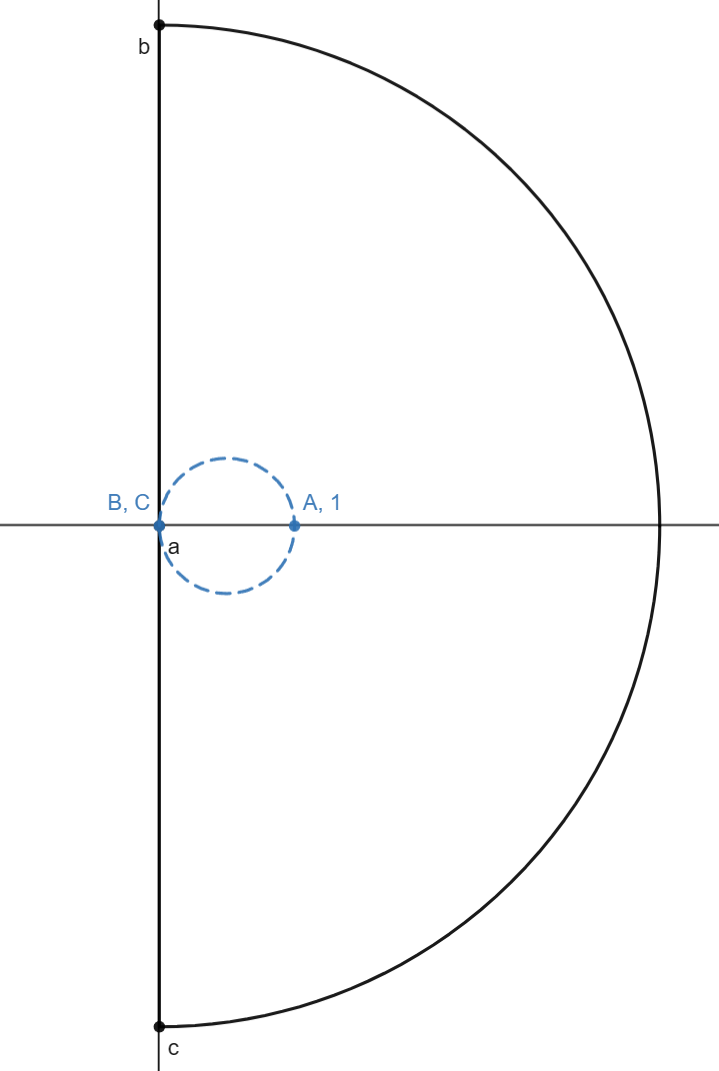
\includegraphics[width=0.3\textwidth]{Questions/Figures/Q1Sketch.png}
    \caption{1(a) Nyquist sketch}
    \label{fig:Q1Sketch}
\end{figure}

\subsection{}
The following MATLAB commands were used to generate the Nyquist plot:
\begin{lstlisting}[language=Matlab]
nyquist(tf([1], [1 1]))
\end{lstlisting}
\begin{figure}[h]
    \centering
    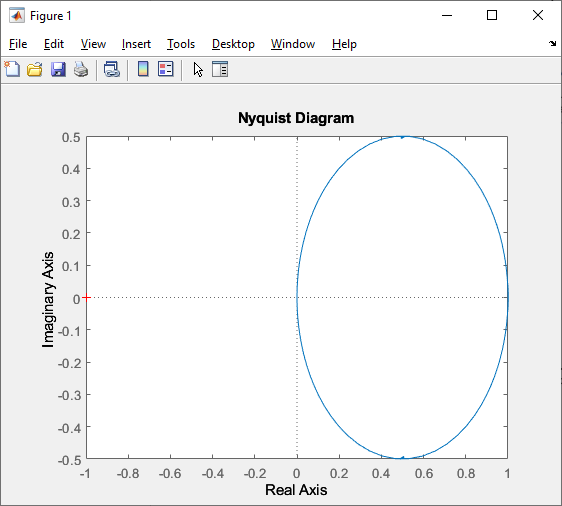
\includegraphics[width=0.5\textwidth]{Questions/Figures/Q1Matlab.png}
    \caption{1(b) Nyquist plot generated by MATLAB}
\end{figure}

\subsection{}
$L(s)$ has no poles in the right half plane, so $n = 0$. Since the Nyquist plot does not pass through $-1$ and encircles
the origin $n=0$ times, the closed-loop system is stable.

\subsection{}
The characteristic polynomial of the closed-loop system is given by
\begin{equation*}
    p(s) = n_p n_c + d_p d_c = 1 + (s+1) = s + 2
\end{equation*}
By Theorem 4.4.1, the closed-loop system is stable if and only if $p(s)$ has negative real roots. Since $p(s)$ has a single
at $s = -2$, the closed-loop system is stable. This matches with the result from (c).